\documentclass[journal,12pt]{IEEEtran}
\usepackage{graphicx} % Required for inserting images
\usepackage{mathpazo} % Palatino font
\usepackage{ragged2e} % Justification package
\usepackage{amsmath}
\usepackage{enumitem} % Enumerate in roman/alphabets etc
\usepackage{titlesec} % Edit section font 
\usepackage{tabularx} % Table with adjustable column width
\usepackage{tikz} % Required for creating diagrams
\usepackage{circuitikz}
\usepackage{karnaugh-map}

\usetikzlibrary{shapes.gates.logic.IEC, positioning}
\renewcommand{\arraystretch}{1.5} % Adjust the value as needed

\titleformat{\section}{\normalfont\bfseries\filright}{\thesection}{1em}{\MakeUppercase}

\begin{document}
\onecolumn

\title{Assembly}
\author{\IEEEauthorblockN{Shreyas Kumar}}
\maketitle
\vspace{-110pt}
\begin{center} shreyas.kumar@icloud.com \end{center}
\vspace{-20pt}
\begin{center} IIT-H Future Wireless Communication \end{center}
\tableofcontents
\section{Question}
\vspace{-30pt}
\begin{flushleft}
$A = a_{1}a_{0}$ and $B = b_{1}b_{0}$ are two 2-bit unsigned binary numbers. If $F(a_{1},a_{0},b_{1},b_{0})$ is a Boolean function such that $F = 1$ only when $A > B$, and $F = 0$ otherwise, then $F$ can be minimized to the form 
\end{flushleft}
\begin{enumerate}[label=\roman*.,labelindent=\parindent,leftmargin=*]
    \item ${a_1}\overline{b}_1 + {a_1}{a_0}\overline{b}_0$
    \vspace{4pt}
    \item ${a_1}\overline{b}_1 + {a_1}{a_0}\overline{b}_0 + {a_0}\overline{b}_0\overline{b}_1$
    \vspace{4pt}
    \item ${a_1}{a_0}\overline{b}_0 + {a_0}\overline{b}_0\overline{b}_1$
    \vspace{4pt}
    \item ${a_1}\overline{b}_1 + {a_1}{a_0}\overline{b}_0 + {a_0}\overline{b}_0{b}_1$
\end{enumerate}
\vspace{80pt}
\section{Truth Table}
\vspace{-1pt}
\begin{center}
  \begin{tabularx}{0.46\textwidth} { 
  | >{\centering\arraybackslash}X 
  | >{\centering\arraybackslash}X 
  | >{\centering\arraybackslash}X
  | >{\centering\arraybackslash}X 
  | >{\centering\arraybackslash}X 
  | >{\centering\arraybackslash}X 
  | >{\centering\arraybackslash}X 
  | >{\centering\arraybackslash}X 
  | >{\centering\arraybackslash}X 
  | >{\centering\arraybackslash}X | }
\hline
${a_1}$ & ${a_0}$ & ${b_1}$ & ${b_0}$ &\textbf{F}\\
\hline
0 & 0 & 0 & 0 & 0  \\  
\hline
0 & 0 & 0 & 1 & 0  \\  
\hline
0 & 0 & 1 & 0 & 0  \\  
\hline
0 & 0 & 1 & 1 & 0  \\  
\hline
0 & 1 & 0 & 0 & 1  \\  
\hline
0 & 1 & 0 & 1 & 0  \\  
\hline
0 & 1 & 1 & 0 & 0  \\  
\hline
0 & 1 & 1 & 1 & 0  \\  
\hline
1 & 0 & 0 & 0 & 1  \\  
\hline
1 & 0 & 0 & 1 & 1  \\  
\hline
1 & 0 & 1 & 0 & 0  \\  
\hline
1 & 0 & 1 & 1 & 0  \\  
\hline
1 & 1 & 0 & 0 & 1  \\  
\hline
1 & 1 & 0 & 1 & 1  \\  
\hline
1 & 1 & 1 & 0 & 1  \\  
\hline
1 & 1 & 1 & 1 & 0  \\  
\hline
\end{tabularx} \\
\vspace{6pt}
\textit{Truth table for Boolean function 'F' } 
\end{center}

\section{Logical Diagram}
\vspace{20pt}
\begin{center}
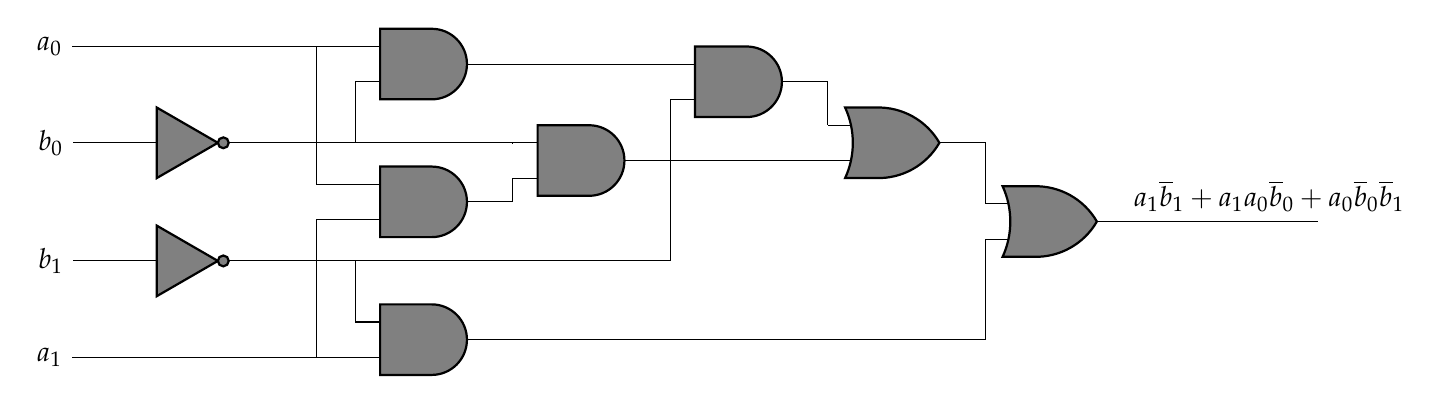
\begin{tikzpicture}
\ctikzset{
    logic ports=ieee,
    logic ports/scale=0.8,
    logic ports/fill=gray
}
 
% Logic ports

\node[not port] (notb1) at (-1,-3.5){};
\node[not port] (notb0) at (-1,-2){};
\node[and port] (andU) at (2,-1){};
\node[and port] (andM) at (2,-2.75){};
\node[and port] (andD) at (2,-4.5){};
\node[and port] (andX) at (6,-1.225){};
\node[and port] (andY) at (4,-2.225){};
\node[or port]  (orX) at (8,-2){};
\node[or port]  (orY) at (10,-3){};

\draw (notb0.out) -| (andU.in 2);
\draw (notb0.out) -| (andY.in 1);
\draw (notb1.out) -| (andD.in 1);
\draw (notb1.out) -| (andX.in 2);
\draw (andM.out) -| (andY.in 2);
\draw (andU.out) -| (andX.in 1);
\draw (andX.out) -| (orX.in 1);
\draw (andY.out) -| (orX.in 2);
\draw (andD.out) -| (orY.in 2);
\draw (orX.out) -| (orY.in 1);
\draw (andM.in 1) -| ++(-0.5,0) |- (andU.in 1);
\draw (andM.in 2) -| ++(-0.5,0) |- (andD.in 2);

\draw (orY.out) -- ++(2.5,0) node[near end,above]{${a_1}\overline{b}_1 + {a_1}{a_0}\overline{b}_0 + {a_0}\overline{b}_0\overline{b}_1$};

\draw (andU.in 1) -- ++(-3.6,0)node[left]{${a_0}$};
\draw (andD.in 2) -- ++(-3.6,0)node[left]{${a_1}$};
\draw (notb1.in 1) -- ++(-0.75,0)node[left]{${b_1}$};
\draw (notb0.in 1) -- ++(-0.75,0)node[left]{${b_0}$};

\end{tikzpicture}
\end{center}

\section{Components}
\vspace{20pt}
\begin{center}
\begin{tabularx}{0.6\textwidth} { 
  | >{\centering\arraybackslash}X 
  | >{\centering\arraybackslash}X 
  | >{\centering\arraybackslash}X
  | >{\centering\arraybackslash}X | }
\hline
\textbf{Component} & \textbf{Values} & \textbf{Quantity} \\
\hline
Arduino & UNO & 1 \\
\hline
Jumper Wires & M-M & 10 \\
\hline
Breadboard & & 1 \\
\hline
LED & & 2 \\
\hline
Resistor & 220 ohms & 1 \\
\hline
\end{tabularx}
\vspace{6pt}
\\\textit{List of items required}
\end{center}


\section{K-map Implementation}
\vspace{10pt}
\begin{flushleft}
Using the boolean logic output F can be expressed in terms of the inputs X,Y,Z with the help of the following Kmap.
\\
\end{flushleft}
\begin{center}
\begin{karnaugh-map}[4][4][1][${b_1}{b_0}$][${a_1}{a_0}$]

    \maxterms{0,1,2,3,5,6,7,10,11,15}
    \minterms{4,8,9,12,13,14}

    \implicantedge{12}{12}{14}{14}
    \implicant{9}{12}
    \implicant{4}{12}
\end{karnaugh-map}
\\
\vspace{-10pt}
\begin{flushleft}
Karnaugh map simplification results in ${a_1}\overline{b}_1 + {a_1}{a_0}\overline{b}_0 + {a_0}\overline{b}_0\overline{b}_1$
\end{flushleft}
\end{center}


\section{Implementation}
\vspace{20pt}
\begin{center}
  \begin{tabularx}{0.46\textwidth} { 
  | >{\centering\arraybackslash}X 
  | >{\centering\arraybackslash}X 
  | >{\centering\arraybackslash}X  | }
\hline
\textbf{Arduino PIN} & \textbf{INPUT} & \textbf{OUTPUT} \\ 
\hline
\textbf 2 & a0 & \\
\hline
\textbf 3 & a1 & \\
\hline
\textbf 4 & b0 & \\
\hline
\textbf 5 & b1 & \\
\hline
\textbf 8 & & F \\
\hline
\end{tabularx}
\vspace{6pt}
\\\textit{Connections}
\end{center}

\begin{flushleft}

Procedure:\\
\begin{enumerate}[label=\alph*.,labelindent=\parindent,leftmargin=*]
    \item Connect the circuit as per the above table.
    \vspace{2pt}
    \item Connect the output pin to LED.
    \vspace{2pt}
    \item Connect inputs to Vcc for logic 1, ground for logic 0.
    \vspace{2pt}
    \item Execute the circuit using the below code.
    \\
    \vspace{7pt}
    \begin{tabularx}{0.56\textwidth} { 
    | >{\centering\arraybackslash}X |}
    \hline
    https://github.com/shr-eyas/FWC/blob/main/Assembly/assembly.asm\\
    \hline
    \end{tabularx}
    \\
    \vspace{10pt}
    \item Change the values of X, Y, Z in the code and verify the truth table.\\
    
\end{enumerate}
\end{flushleft}

\bibliographystyle{ieeetr}
\end{document} 8
